\chapter{UCSB International Capture The Flag}
In diesem Kapitel wird auf den Hacker-Wettbewerb UCSB International Capture The Flag (iCTF) eingegangen. Zuerst wird Allgemeines dazu erläutert. Anschließend wird der zu erstellenden Service beschrieben. Im letzten Abschnitt wird anschließend auf die Durchführung des Wettkampfes eingegangen.

\section{Allgemeines}
Der iCTF wird jährlich von der University of California, Santa Barbara (USCB) veranstaltet und ist der größten Hackerwettbewerbe dieser Art. 
Der iCTF integriert Angriff und Verteidigung zugleich. Die Teilnehmer müssen gleichzeitig Flaggen von fremden Servicen erhalten, sowie ihre eigenen Service patchen um diese nicht mehr angreifbar zu machen.

\section{Service}
In diesem Abschnitt wird der Service für den iCTF erläutert. Dazu wird zuerst auf die Anforderungen eingegangen. Danach wird die Idee beschrieben. Zuletzt wird der Aufbau und die grundlegende Umsetzung dargestellt

\subsection{Anforderungen}
Zuerst mussten die Anforderungen für den Service definiert werden. Dazu wurden neben den offiziellen Anforderungen seitens der USCB auch eigene Anforderungen vom Projekt Team entworfen.

Um einen Service erfolgreich beim iCTF einreichen zu können mussten verschiedene Punkte beachtet werden:

\begin{enumerate}
\item Es muss eine Service angeboten werden, welcher dem Benutzern eine Funktion anbietet. Hier wurden in einem früheren Wettbewerb zum Beispiel ein Service zum Überprüfen der Temperatur angeboten.
\item Ein weiterer Punkt war die Benutzerinteraktion. Hier wurden den Team zwei Möglichkeiten gegeben. Entweder kann auf den Service über ein Webinterface zugegriffen werden oder über die Konsole.
\item Der Service muss zudem eine Sicherheitslücke besitzen, über welche eine Flag ausgelesen werden kann. 
\item Der letzte Punkt beschreibt das Thema für den aktuellen iCTF. Was dieses Jahr (2015) crowdsourcing evil war.
\end{enumerate}

Weiter wurden auch vom Team Anforderungen an den Service gestellt:
\begin{enumerate}
\item Der Service soll zwei Sicherheitslücken aufweisen. Dadurch wird der Schwierigkeitsgrad und die Dauer erhöht welche zum Hacken benötigt wird.
\item Eine weitere Anforderung seitens des Teams bestand darin, dass der Service eine lustige Funktion bieten soll.
\item Zuletzt sollten der Service möglichst leicht umgebaut werden können, dass er auch für die Lehre an der Technische Hochschule verwendet werden kann.
\end{enumerate}


\subsection{Idee}
Für den Service wurden zu Beginn verschiedene Ideen diskutiert. Dabei wurde zunächst auf die Funktion des Services eingegangen. Dabei wurden verschiedene Ansätze eingebracht:

\begin{itemize}
\item Labyrinth in einer Bibliothek
\item Kryptologie Aufgaben 
\item Abgaswerte des Volkswagen Konzerns
\end{itemize}

Aus aktuellem Anlass wurde  der letzte Punkt für den Service gewählt.

Hierbei soll ein Konsolen-Service erstellt werden, welcher die Möglichkeit bietet die Fahrgestellnummer zu überprüfen und dem Benutzer gegebenenfalls seinen Abgaswert mitzuteilen. Zudem wurde der Name des Konzerns abgeändert in Folkswagen.
\\

Als weitere Idee wurde angetragen, dass der Service in bayrischem Dialekt benutzt werden soll. Um den internationalen Teilnehmern am iCTF eine Möglichkeit zu geben den Service zu nutzen wurde zudem ein Übersetzer von Bayrisch auf Deutsch angeboten. 

\subsection{Aufbau}
Der Service wurde in zwei Teile aufgeteilt. Der erste Teil behandelt die Überprüfung der Fahrgestellnummer, der andere den Übersetzer.

\begin{figure}[H]
\centering
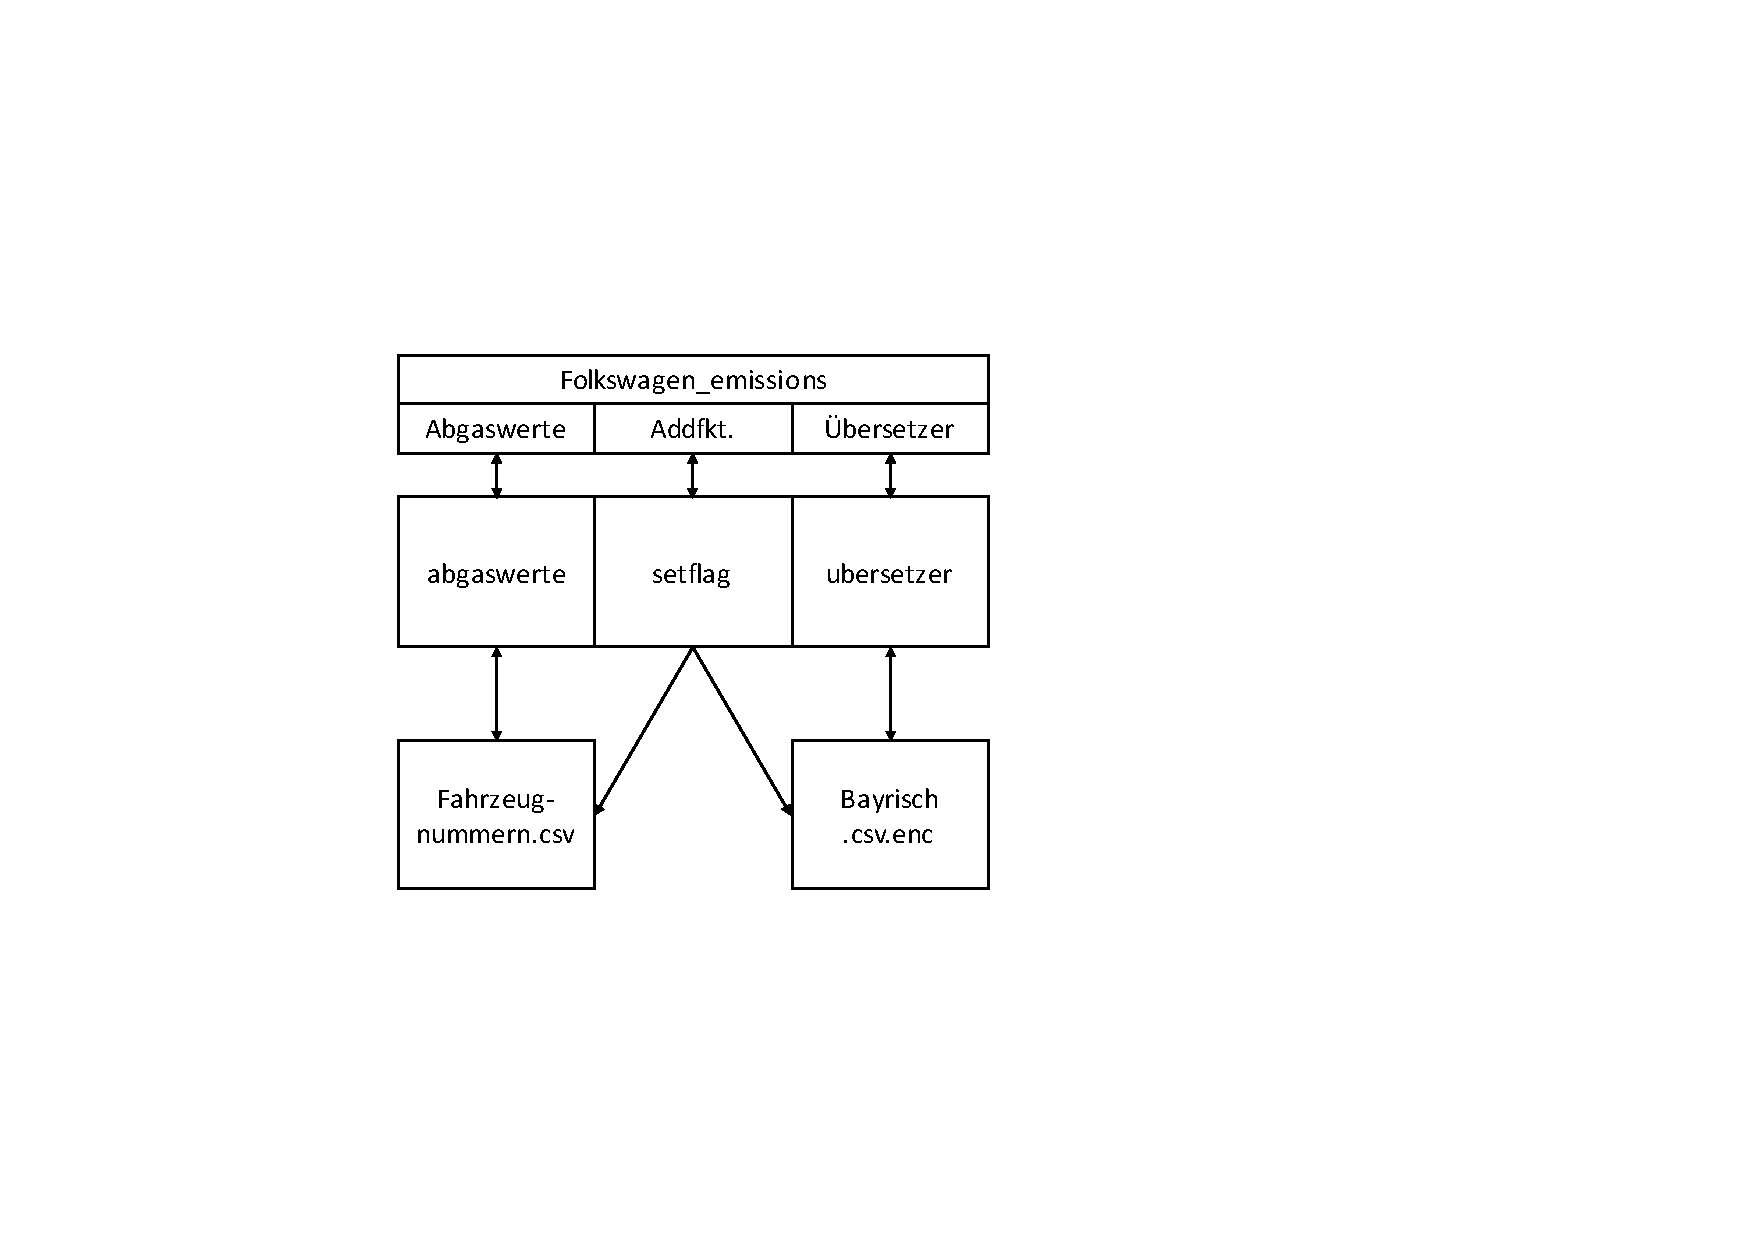
\includegraphics[scale=1]{bilder/ictf/Aufbau_Service.pdf}%
\caption{Service Aufbau}%
\label{serviceAufbau}%
\end{figure}


In Abbildung \ref{serviceAufbau} wird der zweiteilige Aufbau deutlich. Zudem wird das setzen von Flags modelliert. Hierbei handelt es sich um Funktionen für die Organisatoren, welche damit Flags setzen können.
\\

In der linken Hälfte wird der Subservice für die Fahrgestellnummer abgebildet. Dabei wird von der Konsole auf ein Modul \glqq abgaswerte\grqq zugegriffen. Dort werden mithilfe von verschiedenen csv-Dateien die Inhalte der Fahrgestellnummer verarbeitet (Zur Vereinfachung der Darstellung \ref{serviceAufbau} wurden nicht alle csv-Dateien eingezeichnet). Mithilfe dieser Daten kann die Logik entscheiden ob, eine Fahrgestellnummer richtig eingegeben wurde und gibt dann gegebenenfalls einen Abgaswert zurück. \\
Bei dieser Eingabe wird auch die erste Sicherheitslücke implementiert.
\\

In der rechten Hälfte wird der Übersetzer beschrieben. Hierbei wird wiederum über die Konsole auf die Logik zugegriffen. Der Unterschied hierbei ist allerdings, dass der Übersetzer auf eine verschlüsselte Datei zugreift. Diese wurde zum Schutz im voraus vom Projekt-Team entschlüsselt, um sicherheitsrelevante Daten zu schützen und somit die Schwierigkeit des Services zu erhöhen. Beim Zugriff auf die Übersetzungsfunktion wird das csv-File decrypted und das Wort wird in deutscher Sprache zurückgegeben. \\
Auch bei der Eingabe eines bayrischen Wortes ist eine Sicherheitslücke umgesetzt.
\\

Für das Encrypten wurde auch ein eigenes Programm entwickelt. Dieses ist jedoch nicht Bestandteil des Services sondern wurde im Vorfeld entwickelt und verwendet.

\subsection{Sicherheitslücken}
In diesen Abschnitt werden die beiden Sicherheitslücken erläutert. 

\begin{figure}[H]
\centering
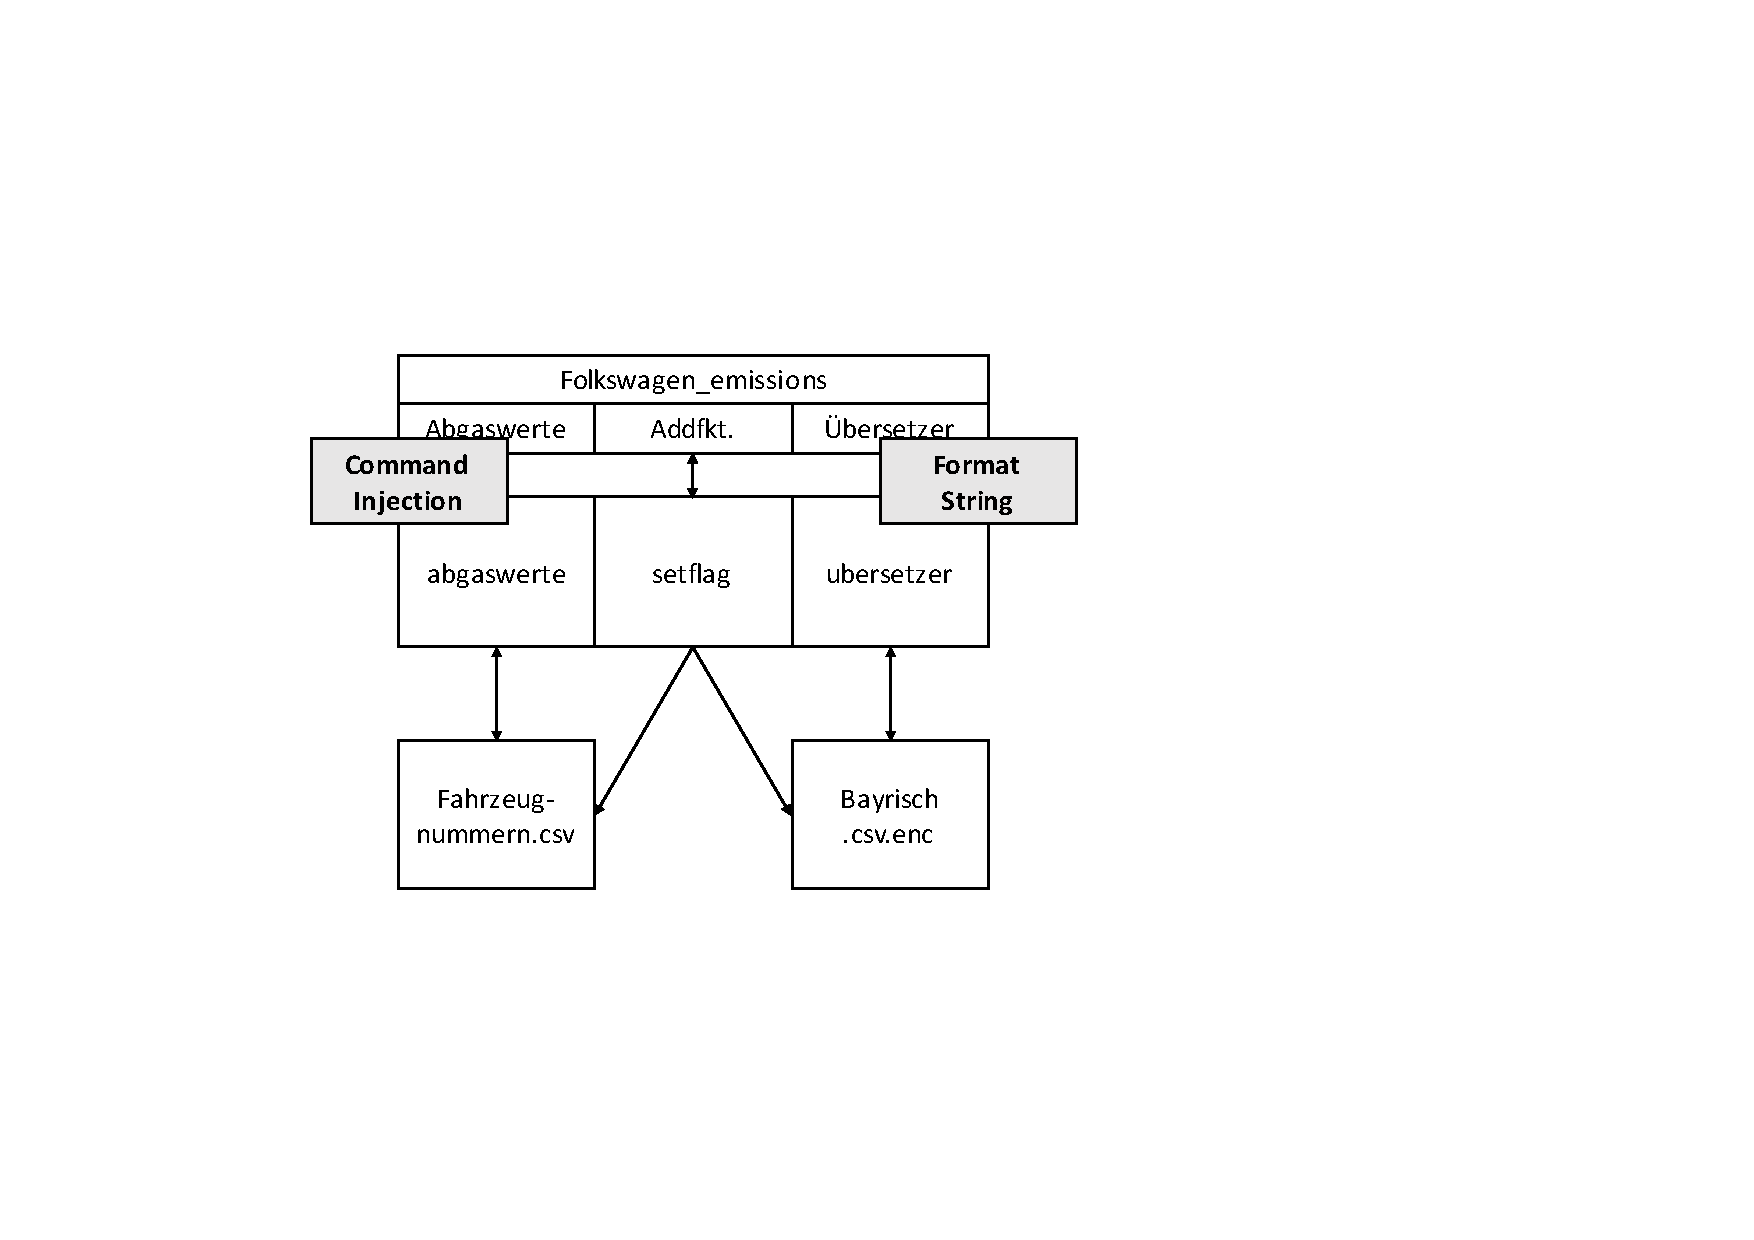
\includegraphics[scale=1]{bilder/ictf/Aufbau_Service_Luecken.pdf}%
\caption{Service Aufbau mit Sicherheitslücken}%
\label{serviceAufbauLuecken}%
\end{figure}

Wie in der Abbildung \ref{serviceAufbauLuecken} zu sehen ist, wurden in jedem Subservice eine Sicherheitslücke eingebaut. 

\subsubsection{Command Injection - Abgaswerte}
Im Abgas Teil wurde eine Command Injection eingebaut. Mithilfe dieser Sicherheitslücke kann auf was Dateisystem zugegriffen werden.
Da die Eingabe direkt auf dem Betriebssystem ausgeführt wird kann durch anhängen von Konsolen-Kommandos im Zielsystem navigiert und agiert werden. 
Dies kann durch unterschiedliche Pattern erzwungen werden:
\begin{itemize}
\item |
\item || 
\item ; 
\item \&\& 
\end{itemize}

All diese Pattern führen die angehängten Befehle aus und geben den Inhalt zurück. Dadurch kann über das Dateisystem auf die Fahrzeugnummern.csv zugegriffen und der Inhalt ausgelesen werden. 

\subsubsection{Formatstring-Angriff - Übersetzer}
Der Übersetzer wurde mithilfe von Formatstring angreifbar gemacht. Dabei können Informationen welche auf dem Stack liegen ausgelesen werden.
Um diese Lücke zu benutzen, muss im Übersetzer mithilfe der Token \%x oder \%s der Speicherinhalt auf der Konsole ausgegeben werden. Die Ausgabe muss anschließende nur noch umgewandelt werden. Somit kann hier der Inhalt der encrypteten Bayrisch.csv ausgelesen werden.
\\

Mithilfe dieser Informationen kann nun eine Flag erzeugt und beim Veranstalter eingereicht werden.
\subsection{Umsetzung}
Zuletzt wird auf die Umsetzung eingegangen. Dabei müssen drei Teile betrachtet werden. Die Oberfläche, die Abgaswerteprüfung und er Übersetzer. Zudem wird auf Umsetzung sonstiger Files eingegangen.

\subsubsection{Oberfläche}
Da die Oberfläche eine einfache Konsole ist wurde hierzu ein Python Skript entworfen, welches einen Socket implementiert. In diesem Skript wird die Interaktion mit dem Benutzer modelliert. Durch eingaben in die Konsole kann der Nutzer sich durch die verschiedenen Funktionen navigieren. So kann er zum Beispiel über den Befehlt \glqq I ko koa bayrisch\grqq  den Übersetzer starten.

\subsubsection{Abgaswerte}
Als nächstes wird auf die Umsetzung der Abgaswerteprüfung eingegangen. Dafür wurde ein C-Programm entwickelt. Die Programmiersprache C wurde gewählt, da dadurch der Code nicht eingesehen werden kann. 
\\

Bei dieser Funktion wird als Eingabe eine Fahrgestellnummer erwartet. Diese wird anschließend überprüft ob diese richtig ist. Stimmt sie mit dem Pattern überein wird ein Abgaswert aus der Fahrzeugnummern.csv ausgelesen. 
Wird eine Command Injection ausgeführt, werden hier zudem die Pattern gefiltert und der Zugriff kann ausschließlich durch \glqq \&\&\grqq durchgeführt werden.

\subsubsection{Übersetzer}
Zuletzt wird der Übersetzer beschrieben. Auch hier wurde aus den gleichen Gründen wie bei den Abgaswerten ein C-Programm entwickelt.
\\

In diesem Modul wird ein bayrisches Wort übergeben und anschließend verarbeitet. Dazu wird zunächst die encryptete Bayrisch.csv-Datei decryptet. Dabei wird der Inhalt auf den Stack geschrieben, was Grundlage für den Zugriff auf die Informationen ist. Anschließend wird überprüft, ob das Wort übersetzt werden kann. Ist dies der Fall, wird das deutsch Wort an den Benutzer zurückgegeben.

\subsubsection{Sonstiges}
Es wurden auch noch weitere Files angelegt. 
Dazu gehören unter anderem die setFlag und getFlag Funktionen. Diese wurden vom Veranstalter gefordert und verwalten die Verteilung der Flags an die Teilnehmer.
\\

Des weiteren wurde ein Exploit für den eigenen Service geschrieben welcher. Mit diesem Skript ist es möglich den Service automatisiert anzugreifen. Dadurch kann zudem einfach nachvollzogen werden welche Schritte gemacht werden müssen um an die Flag zu gelangen. Auch dieses File musste beim Veranstalter eingereicht werden.
\\

Zuletzt wurden noch csv-Datein erstellt, welche die Inhalte des Übersetzers, der Fahrgestellnummer und der Abgaswerte speichern. Diese werden von dem jeweiligen Subservice genutzt.


\section{Der iCTF 2015}
In diesem Kapitel wird auf den iCTF 2015 eingegangen. Dazu wird zuerst Allgemeines vom Event berichtet. Anschließend werden auf die Lessons Learned eingegangen.

\subsection{Allgemeines}
Dieses Jahr fand der Wettbewerb am 04.12. statt und ca. 40 Teams nahmen daran Teil. Dabei belegte unser Team (in23canation) den 22. Platz. Die Dauer des Wettbewerbs wurde mit 24 Stunden angekündigt jedoch kurz vor dem iCTF auf 8 Stunden reduziert. 
Die Stimmung beim Wettbewerb war durchgehend positiv und insgesamt war der CTF ein großer Erfolg. Durch etwas Werbung vorab war es möglich eine große Teilnehmerzahl aus allen Semestern zu begeistern sich unserer Gruppe anzuschließen. Schon bei den zwei vorangehenden Informationsveranstaltungen waren über 60 Studenten anwesend. Beim iCTF selber waren rund 25 Teilnehmer aktiv dabei. 

\subsection{Lessens Learned}
Nach der Durchführung des iCTFs konnten einige Punkte festgehalten werden welche bei zukünftigen Ereignissen beachtet werden sollten. 
Diese werden im folgenden aufgelistet:

\begin{enumerate}
\item Es muss vor dem Event ein sicheres, vom Hochschulnetzwerk getrenntes Netzwerk für den Wettbewerb eingerichtet werden
\item Gesonderter Backup von jedem Service um Probleme beim Patchen schnell rückgängig zu machen
\item Mehrere Zugriffe auf das iCTF-Netzwerk um einen Flaschenhals zu vermeiden
\item Skripte zum einreichen der Flags können im voraus fertiggestellt werden
\item VM mit Etterpad und Fileshare vorbereiten und einmal einrichten um Problemen vorzubeugen 
\item Nginx Konfiguration vorbereiten
\item Live Chats vom Veranstalter von Beginn an verfolgen um keine Ankündigungen zu verpassen
\item Zutritt zur Hochschule ist Samstags gesondert einzurichten  
\end{enumerate}





